\documentclass{amsart}
\usepackage{mathpazo, enumitem}
\usepackage{tikz}
\usepackage{graphicx}
\title{Problem Set 1 Solutions}
\begin{document}
\maketitle

\section*{Question 1}

Define an isomorphism of graphs.  Which of the following graphs are isomorphic?  Justify your answer.  

  \includegraphics[width=.9\textwidth]{FourGraphs.png}

\subsection*{Definition of an Isomorphism}

    An isomorphism between two \emph{simple} graphs $G$ and $H$ is a bijection $\varphi:V(G)\to V(H)$ so that for all $v, w\in V(G), \varphi(v)$ and $\varphi(w)$ are adjacent if and only if $v, w$ were.  Alternatively, this can be phrased as: $\varphi$ preserves the number of edges between vertices.

\subsection*{Commentary on the definition}    
    Note that we required the graph to be simple: if $G$ has multiple edges or loops, then our definition of isomorphisms need to keep track of some extra information.  This won't appear on the exam, but it is instructive to try to understand yourself: the graph $G$ with one vertex and one loop (an edge) should have two different isomorphisms from $G$ to itself; the graph $H$ with two vertices and two edges between them should have 4 different isomorphisms from $H$ to itself.

\subsection*{Showing Graph 2 and Graph 4 aren't isomorphic to 1 and 3}
A common confusion about the four graphs was that people only looked at the isomorphisms that preserved the labelling of the vertices -- that is, only looked at the map $\varphi$ with $\varphi(a)=a, \varphi(b)=b$, etc.  This confusion is understandable, but the labellings don't in general need to be preserved; they're just there so we have a way to write down what the map $\varphi$ is.

    As for the four graphs: the first thing to do is look at the number of vertices and their degrees -- we see all that all four graphs have 8 vertices, but that Graph 4 has vertices of degree 4 while none of the other graphs do (Graph 4 actually has more edges than the other graphs).  So, we see immediately that Graph 4 cannot be isomorphic to any of the others.

    Next we look for other invariants of the graphs -- the lengths of cycles is a good one, and we see that while Graph 2 is bipartite, and hence only has cycles of even length, Graph 1 and Graph 3 are not -- they have no triangles, but they have cycles of length 5.  (Note a few of you got confused about this -- where the edges cross is not a vertex).


\subsection*{Longwinded discussion about how you might look for an isomoprhism between Graph 1 and Graph 3}    
    Graph 1 and Graph 3 are isomorphic; there are lots of different isomorphisms between them, because Graph 1 (and hence Graph 2) is highly symmetric.  Rather than just write one down, I will walk you through the thought process that might lead you to discover an isomorphism between the two graphs.

    Looking at Graph 1, we note that ``every vertex looks the same'' -- just rotate the octagon a bit (more precisely, ``the automorphism group of Graph 1 acts transitively on the vertices'' -- for any two vertives $v$ and $w$, there is an isomorphism $\varphi$ from Graph 1 to itself with $\varphi(v)=w$).

    Thus, Graph 1 and Graph 3 were isomorphic, we send any vertex of Graph 1 to Graph 3 -- in particular, there would be an isomorphism with $\varphi(a)=a$.

    Now, the three edges out of $a$ in Graph 1 would have to go to the three edges out of $a$ in Graph 3 -- could we do this any way we choose, or do some edges ``look different'' than other edges?  Intuitively, looking at Graph 1 the edges around the outside of the octagon are different than the edges going across the middle (more precisely, there are not isomorphisms from Graph 1 to itself that change one type of edge for the other).

    How can we make precise the notion that $ae$ is ``different'' from $ab$ or $ah$?  Well, Graph 1 has 4 different four cycles, the bowties through the middle, like $aefba$.  The edges around the outside octagon are in precisely 1 of these four cycles, while the edges across the middle are in two different four cycles -- e.g., $ae$ is in both $aefba$ and $aedha$.  If Graph 1 and Graph 3 are isomorphic, something similar must be true there.

    Indeed, we see that Graph 3 has 4 different 4-cycles: $abcda, aehda, fbcgf$, and $egfhe$.  The edges that are in two different four cycles in Graph 3 are precisely the 4 vertical edges: $ad, eh, fg$ and $bc$.  Thus, we see the four edges across the middle of Graph 1 are going to have to map to the four vertical edges in Graph 3.  In particular, if $\varphi(a)=a$, then we need $\varphi(e)=d$, so that $ae$ maps to $ad$.

    Note that the map that reflects across the edge $ae$ is an isomorphism of Graph 1, so even having fixed that $\varphi(a)=a$, we still have that $b$ and $h$ look interchangeable, and so we could send either one of these vertices to $b$ in Graph 3; we will send $\varphi(b)=b$, and hence we must have $\varphi(h)=d$.

    At this point the rest of the isomorphism $\varphi$ is fixed, working out vertex by vertex like this.  An easy way to see this is if we delete the four edges across the middle in Graph 1, we are left with an 8 cycle, and if we delete the four vertical edges in Graph 3 we also have an 8 cycle, $abfhdcgea$.  Preserving these cycles in this order gives an isomorphism between the graphs (you should check it maps the edges across the middle to the vertical edges).

    \subsection*{The actual isomorphism written down, which is all the question needed}
    $$\begin{tabular}{c|c|c|c|c|c|c|c}
      a & b & c & d & e & f & g & h \\ \hline
  a& b & f & h & d & c & g & e
    \end{tabular}$$


    
\section*{Question 2}

\begin{enumerate}[label=\alph*)]
\item  Define what it means for a graph to be Eulerian, semi-Eulerian, Hamiltonian, and semi-Hamiltonian.
\item Give an example of a graph with 5 vertices such that $G$ is Hamiltonian but not semi-Eulerian.  Justify that $G$ has these properties.
\item Give an example of a graph with 5 vertices such that $G$ is Eulerian but not semi-Hamiltonian.  Justify that $H$ has these properties.
\end{enumerate}

\subsection*{The straightforward definitions}
An \emph{Eulerian cycle} is a closed walk that uses every edge of $\Gamma$ exactly once; an \emph{Eulerian path} a walk that uses every edge of $\Gamma$ exactly once. A \emph{Hamiltonian cycle} is a closed walk that uses every vertex exactly once; a \emph{Hamiltonian path} is a walk that uses every vertex exactly once.

A graph is \emph{Eulerian} if it has an Eulerian cycle, and \emph{Hamiltonian} if it has a Hamiltonian cycle.  

\subsection*{The definitions I messed up}

It is slightly less clear what should be meant when for the "semi" variations.  The point is that a semi-Eulerian graph should have an Eulerian walk, and a semi-Hamiltonian walk should have a Hamiltonian walk.  The only question is that some sources explicitly a semi-Eulerian graph from being Eulerian, and a semi-Hamiltonian graph from being Hamiltonian, while others allow it.  When I wrote the notes a long time ago I looked up what the more standard convention seemed to be and used that, but in lecture I forgot about this and used what seems more natural to me.

\subsubsection*{Inclusive definitions}

The definitions I actually prefer are:

A graph is \emph{semi-Eulerian} if it has a (not necessarily closed) walk that uses every edge exactly once. A graph is \emph{semi-Hamiltonian} if it has a (not necessarily closed) walk that uses every vertex exactly once.

\subsubsection*{The exclusive definitions}

The definition you'd find on wikipedia, and that past Paul copied into the notes and then forgot:

A graph is \emph{semi-Eulerian} if it has an Eulerian path but \emph{not} an Eulerian cycle.  A graph is \emph{semi-Hamiltonian} if it has a Hamiltonian path but \emph{not} a Hamiltonian cycle.

\subsubsection*{The definition you don't want}

Not that since there is this ambiguity, whatever definition you use, you want to address it; you don't want something that is unclear.  So, just saying ``A graph is semi-Eulerian if it has an Eulerian path'' isn't great, as it's not clear what if an Eulerian graph would be considered semi-Eulerian or not.  Also, whatever definition you wrote down, the example graph you gave should work \emph{for that definition}; a few people wrote down one definition, and then gave an example that only worked for the other definition.

\subsection{Making lemonade from lemons}
While I apologize for the confusion in this definition, I think some meta-discussion about definitions and conventions like this is a valuable thing to have.

This kind of slight variance in definition and convention is rather commonplace, and in writing formal math it's usually a good idea to recall the definitions you're using, just in case somebody else has used a slightly variant definition and it winds up mattering.


\subsubsection*{Definitions and the exam}

For the course, I'm not too wedded to these definitions.  In a lot of situations the difference in definitions doesn't matter, and if I just ask you for the definition I would except either one.  If there is a situation in which it's important which definition is being used, I will be sure that there is some explicit cue that tells you which definition is being used.

\subsection*{The example graphs}

\subsubsection*{The exclusive case is easy}
First note that if we take the \emph{exclusive} definition, then any graph that is both Eulerian and Hamiltonian would work for both parts b) and c) Since it is Hamiltonian, it would not be semi-Hamiltonian, and since it is Eulerian it would not be semi-Eulerian.  So, the 5 cycle $C_5$ or the complete graph $K_5$ would work.

\subsubsection*{The inclusive case is a bit harder}
Now we construct examples if we take the inclusive definition.

We want $\Gamma$ to be Hamiltonian, so let's begin by drawing a Hamiltonian cycle.

In lecture we proved the following variant of Euler's theorem: if at most two vertices have degree 2, then $\Gamma$ has an Eulerian path.  Since a graph has to have an even number of vertices of degree, we need to have four vertices of odd degree.  Every vertex already has degree 2 because of the Hamiltonian cycle; if we only have five vertices, the highest the degree of any vertex can get (if we want a simple graph) is 4, then the only option is to have 4 vertices of degree 3, which produces this graph:
\begin{center}
\begin{figure}
  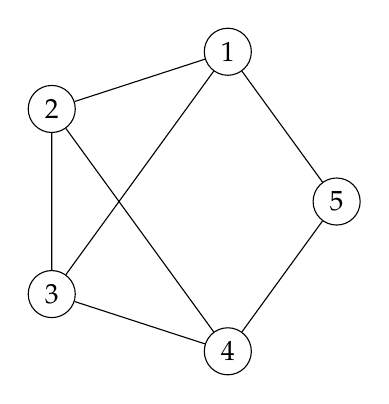
\begin{tikzpicture}
\tikzstyle{vertex}=[circle, draw, minimum size=17pt, inner sep=0pt]
\foreach \x in {1,2,...,5} {
  \node[vertex] (\x) at (72*\x:2) {\x};}
\draw (1)--(2)--(3)--(4)--(5)--(1)--(3);
\draw (2)--(4);
\end{tikzpicture}
  \caption{A graph that is Hamiltonian but not semi-Eulerian}
  \end{figure}
\end{center}


To be Eulerian, every vertex has to have even degree, namely 0, 2 or 4.  If we want a \emph{simple} graph, I don't believe we can make a \emph{connected} graph be Eulerian but not semi-Hamiltonian in the inclusive sense with only 5 vertices, but disconnected graphs are never semi-Hamiltonian and so something like this is the easiest example. 
If we allow multiple edges, then many possibilities are available: take any non-semi-Hamiltonian graph, and add multiple edges until all vertices have even degree.
\begin{figure}

  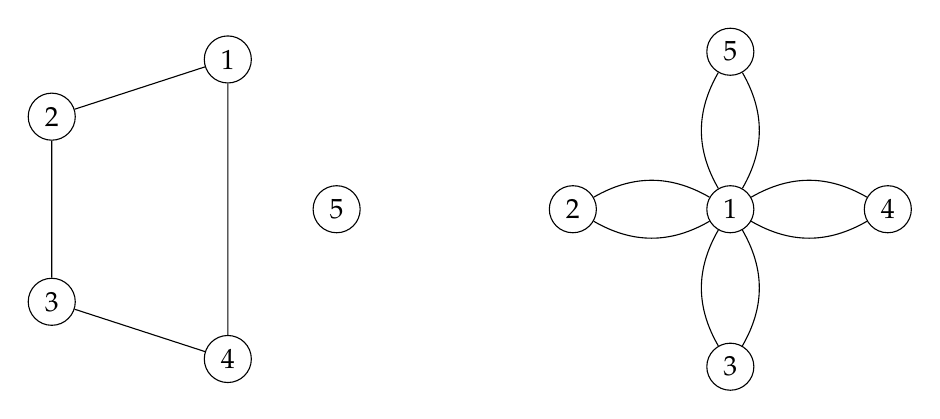
\begin{tikzpicture}
\tikzstyle{vertex}=[circle, draw, minimum size=17pt, inner sep=0pt]
\begin{scope}
\foreach \x in {1,2,...,5} {
  \node[vertex] (\x) at (72*\x:2) {\x};}
\draw (1)--(2)--(3)--(4)--(1);
\end{scope}

\begin{scope}[xshift=7cm]
\foreach \x in {2,...,5} {
  \node[vertex] (\x) at (90*\x:2) {\x};}
\node[vertex] (1) at (0,0) {1};
\draw (1) to [bend left] (2);
\draw (2) to [bend left] (1);
\draw (1) to [bend left] (3);
\draw (3) to [bend left] (1);
\draw (1) to [bend left] (4);
\draw (4) to [bend left] (1);
\draw (1) to [bend left] (5);
\draw (5) to [bend left] (1);
\end{scope}
  \end{tikzpicture}
  \caption{Two graphs that are Eulerian but not semi-Hamiltonian}
  \end{figure}

For completeness, the following simple, connected graph on \emph{six} vertices is Eulerian but not semi-Hamiltonian (prove it!)

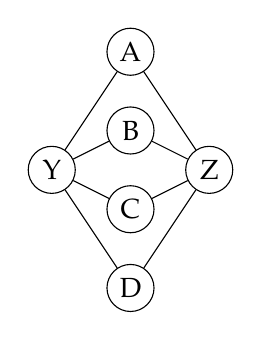
\begin{tikzpicture}
\tikzstyle{vertex}=[circle, draw, minimum size=17pt, inner sep=0pt]
  \node[vertex] (Y) at (0,0) {Y};
\node[vertex] (Z) at (2,0) {Z};
\node[vertex] (A) at (1, 1.5) {A};
\node[vertex] (B) at (1, .5) {B};
\node[vertex] (C) at (1,-.5) {C};
\node[vertex] (D) at (1,-1.5) {D};

\draw (Y)--(A)--(Z)--(B)--(Y);
\draw (Y)--(C)--(Z)--(D)--(Y);
\end{tikzpicture}

\section*{Question 3}


Given that Fluorine ($F$) has valency 1, prove that any molecule with formula $C_5H_{11}F$ is a tree.  How many isomers does $C_5H_{11}F$ have?  Draw them.

\subsection*{Prove the molecule is a tree}

To prove that a graph is a tree, it is enough to prove that it is connected, and that it has one less edge than vertex.  Since molecules are by definition connected, we know any isomer of $C_5H_{11}F$ is connected.  It has 5+1+11=17 vertices, so we need to prove it has 16 edges.

Since we know the degree of each vertex, we can count the edges using the handshaking lemma:

$$2e=\sum_{v}d(V)=4\cdot 5+11\cdot 1+1\cdot 1=32$$
and so indeed there are 16 edges.

\subsection{Discussion of common mistakes}
A lot of you either drew one isomer and showed it was a tree, or made some argument about the 4 carbons needing to be connected and that using up only a certain number of edges, and then all the other edges needed to be used to to connect the $H$ and $F$ in and that not leaving another to close up a loop for the carbon.

Neither of these arguments is \emph{wrong}, persay, but I would argue that neither is as good as the proof of the handshaking lemma proof.

For instance, if you just draw one isomer, how do you know that any other isomer would also be a tree?  While it is true that if any one isomer is a tree than all isomers are a tree, I think proving that carefully boils down to using the Handshaking lemma.

And the second argument, you're sort of implicitly using the handshaking argument, and not exactly stating it, and it winds up being more work and not as slick and clean.

\subsection*{Finding the isomers}


To count the isomers, note first that since all the other molecules have degree 1, they are leaves, and deleting them we would still have a tree, so the 5 carbon molecules will make a tree.  There are three possible ways to do this: they can be in a chain of length 5, there can be one carbon connected to three others, or there could be one carbon connecting to 4 others.  

If we were counting isomers of $C_5H_{12}$, as done in class, we would be done; but we have replaced one of the $H$ with $F$, which makes that vertex special.  Hence, if the $F$ is attached to different carbon atoms, we might get different isomers (we may still get isomorphic ones -- for instance, attaching the $F$ to either end molecule of the chain of carbons would result in the same graph).

There are 8 in total, then; in the pictures below we have drawn the Carbons and the Flouride, but the location of the Hydrogen is left implicitly by degree.
\begin{center}
\begin{tikzpicture}[scale=.9]
  \begin{scope}
    \foreach \x in {1,...,5} {
      \node (\x) at (\x,0) {$C$};
    }
    \node (6) at (1,1) {$F$};
    \draw (5)--(4)--(3)--(2)--(1);
    \draw (1)--(6);
  \end{scope}
  \begin{scope}[yshift=-3cm]
    \foreach \x in {1,...,5} {
      \node (\x) at (\x,0) {$C$};
    }
    \node (6) at (2,1) {$F$};
    \draw (5)--(4)--(3)--(2)--(1);
    \draw (2)--(6);
  \end{scope}
    \begin{scope}[yshift=-6cm]
    \foreach \x in {1,...,5} {
      \node (\x) at (\x,0) {$C$};
    }
    \node (6) at (3,1) {$F$};
    \draw (5)--(4)--(3)--(2)--(1);
    \draw (3)--(6);
  \end{scope}

  \begin{scope}[xshift=6cm]
    \node (1) at (1,0) {$C$};
    \node (2) at (2,0){$C$};
    \node (3) at (3,0){$C$};
    \node (4) at (4,.5){$C$};
    \node (5) at (4, -.5){$C$};

    \node (6) at (1,1) {$F$};
    \draw (4)--(3)--(2)--(1);
    \draw (5)--(3);
    \draw (1)--(6);
  \end{scope}

    \begin{scope}[xshift=6cm, yshift=-3cm]
    \node (1) at (1,0) {$C$};
    \node (2) at (2,0){$C$};
    \node (3) at (3,0){$C$};
    \node (4) at (4,.5){$C$};
    \node (5) at (4, -.5){$C$};

    \node (6) at (2,1) {$F$};
    \draw (4)--(3)--(2)--(1);
    \draw (5)--(3);
    \draw (2)--(6);
    \end{scope}

      \begin{scope}[xshift=6cm, yshift=-6cm]
    \node (1) at (1,0) {$C$};
    \node (2) at (2,0){$C$};
    \node (3) at (3,0){$C$};
    \node (4) at (4,.5){$C$};
    \node (5) at (4, -.5){$C$};

    \node (6) at (3,1) {$F$};
    \draw (4)--(3)--(2)--(1);
    \draw (5)--(3);
    \draw (3)--(6);
      \end{scope}

        \begin{scope}[xshift=6cm, yshift=-9cm]
    \node (1) at (1,0) {$C$};
    \node (2) at (2,0){$C$};
    \node (3) at (3,0){$C$};
    \node (4) at (4,.5){$C$};
    \node (5) at (4, -.5){$C$};

    \node (6) at (5,.5) {$F$};
    \draw (4)--(3)--(2)--(1);
    \draw (5)--(3);
    \draw (4)--(6);
  \end{scope}

  \begin{scope}[yshift=-9cm]
    \node (1) at (2,0) {$C$};
    \node (2) at (3,0){$C$};
    \node (3) at (3,1){$C$};
    \node (4) at (3,-1){$C$};
    \node (5) at (4, 0){$C$};

    \node (6) at (1,0) {$F$};
    \draw (6)--(1)--(2)--(3);
    \draw (4)--(2)--(5);
  \end{scope}        

\end{tikzpicture}
\end{center}  




\end{document}
